\section{Verification of the Optimizer}
\label{sec:optimizer-verification}
The reduced models I used are known to be too simple to precisely match all electrophysiological features exhibit by all cell types; this can be an advantage, as this also means that they are too inflexible to fit the ``noise" in the data, whether it be random thermal fluctuations or systematic recording errors.
These latter may be quite common; sites like NeuroElectro control only the extracted data is faithful to that reported in the publication, not that it reflects what was seen in the actual experiments, or that those experiments were carefully performed.
Therefore, if the first step were applying the optimizer to fit models to real biological data, we would have no idea whether any optimization failures (poorly fitting models) reflected the limitations of the biological data, the limitations of the underlying model, or the limitations of the optimizer algorithms.
%And before attempting to identify the magnitude or cause of poor fits, at least four factors that shape optimizer validation and design must be controlled for.
%These are: the informativeness of measurement errors, the performance of the optimizer, the quality of the data, and the quality of the models.

It is therefore necessary to create data-source independent ``ground truths", by simulating data from the models themselves, and using the optimizer to see if those model parameters can be recovered from that simulated data.
Because genetic algorithms (such as the DEAP \citep{DEAP_JMLR2012} implementation used here) has notably good performance in handling complicated error surfaces (such as Rastrigrin's function), I expect that my optimization frame work, which derives from it, should also be able to handle potentially complicated features spaces such as one would expect from the output of a complex dynamical system like a neuron.

I wrote an algorithm that senses the edges of defined model parameter boundaries, and defines uniformly distributed random numbers within those boundaries. Alternatively I could have chosen to draw numbers from uniformly distributed random number generators, but doing so would risk testing only typical optimization cases and excluding edge cases.
% The algorithm I wrote to choose random model parameters samples from uniform distributions across parameter ranges, and the case above, shows a model in a fringe case.


\subsection{Verification Endpoints}
My optimizer was capable of identifying model parameterizations that nearly perfectly matched the parameters of the ``ground truth" models that generated the constraining simulated data (Figure \ref{fig:optimizer-verification-radar}).
Simulated output of the two models matched closely as well (as expected from similar model parameters) (Figures \ref{fig:optimizer-verification-traces-1}, \ref{fig:adexp_model_rebound_spike}, \ref{fig:optimizer-verification-traces-3}).
NeuronUnit-based electrophysiological features extracted from the traces shown in those figures, and from other traces simulated in the course of optimization, also showed a near-perfect match (i.e. Z-score of 0, indicating perfect optimization) (Table \ref{table:optimizer-verification}).

\begin{table}[ht]
\centering
\resizebox{\textwidth}{!}{
\begin{tabular}{|l|l|l|l|}
\toprule
{} &    Observations &     Predictions & Z-Scores \\
\midrule
RheobaseTest         &         1.62 pA &         1.62 pA &        0 \\
TimeConstantTest     &        13.18 ms &        13.18 ms &        0 \\
RestingPotentialTest &       -77.43 mV &       -77.43 mV &        0 \\
InputResistanceTest  &  270.84 megaohm &  270.84 megaohm &        0 \\
CapacitanceTest      &        48.65 pF &        48.65 pF &        0 \\
FITest               &    7.51 Hz/pA &    7.51 Hz/pA &        0 \\
\bottomrule
\end{tabular}}
\caption[Optimizer verification table]{\textbf{``Observed" and ``Predicted" electrophysiological features match to within a few decimal places}.
Here, ``Observed" refers to values extracted from traces simulated from a ground-truth model.
The optimizer has no knowledge of the parameters of that model, but uses these ``Observed features" to attempt to discover them using a genetic algorithm.
The algorithm modified these parameters in order to bring the ``Predicted" features values, extracted from new simulations, in line with the ``Observed" ones.
Each row refers to a distinct NeuronUnit test used to simulate the model, extract a single electrophysiological feature, and compute a Z-score.
The outcome of this algorithm is shown in this table, demonstrating that the optimizer has identified a parameter set that perfectly reproduces these features.}
\label{table:optimizer-verification}
\end{table}

\clearpage
\begin{figure}
    \centering
    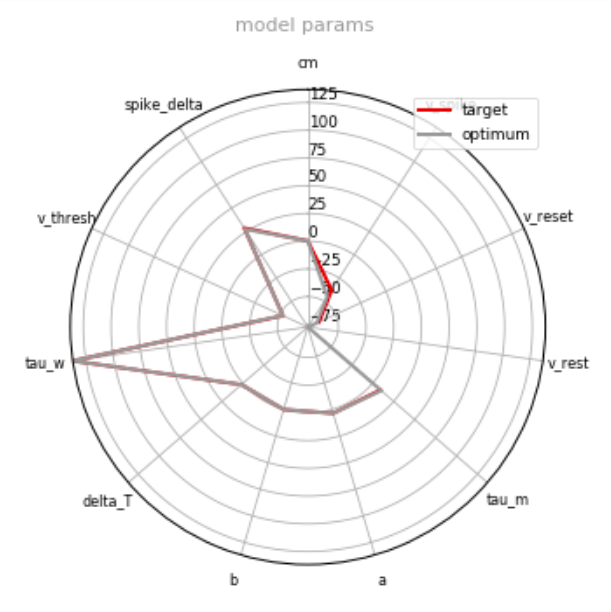
\includegraphics[scale=0.75]{figures/radar_coordinates.png}
    \caption[Radar Plot of Optimizer Verification against Ground Truth]{\textbf{Radar Plot of Optimizer Verification against Ground Truth.}
    ``Target" refers to parameters from the ground-truth model.
    ``Optimum" refers to parameters obtained by the optimizer when trying to match the features shown in Table \ref{table:optimizer-verification}.
    Despite having no knowledge of the ground truth parameters,
    the optimizer can discover them by feature-matching, producing a near perfect match.
    Nearly all of the 11 Izhikevich model parameters are accurately recovered, with only a trivial discrepancy in $v_spike$.
    }
    \label{fig:optimizer-verification-radar}
\end{figure}

\begin{figure}
    \centering
    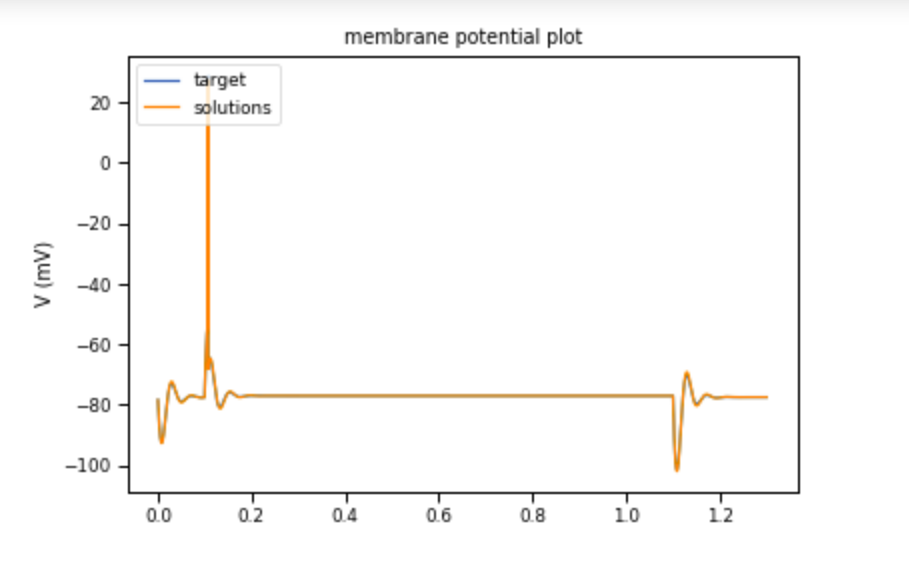
\includegraphics[scale=0.85]{figures/simulated_data_supra_threshold.png}
    \caption[Optimizer Verification Example 1]{\textbf{Optimizer Verification Example 1.} The orange trace shows the model waveform recovered during the process of optimization.
    Blue trace (not visible due to occlusion by orange trace) depicts the simulated trace (in response to the rheobase current) from the ground truth model that were used to guide optimization.
    The horizontal axis shows simulation time in seconds.
    Clear agreement is shown in between simulated responses of the ground truth model and the optimized model from Figure \ref{fig:optimizer-verification-radar}. 
}
\label{fig:optimizer-verification-traces-1}
\end{figure}

\begin{figure}
    \centering
    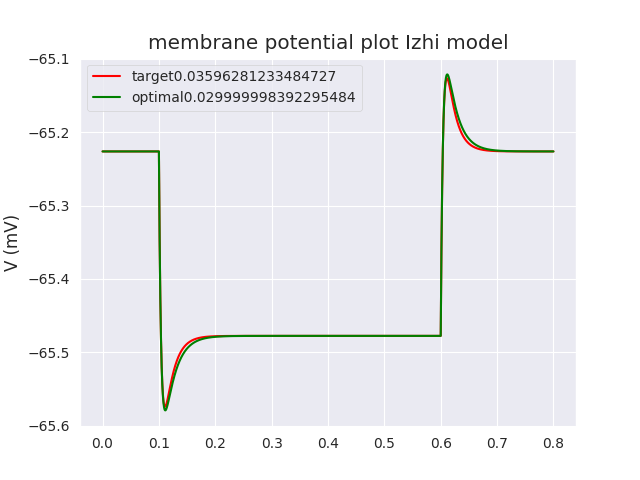
\includegraphics[scale=0.85]{figures/capacitance.png}
    %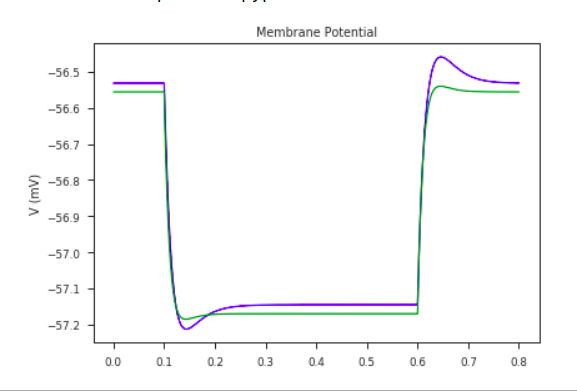
\includegraphics[scale=0.85]{figures/passive_model_agreement}
    \caption[Optimizer verification example 2]{
    Similar to Figure
    \ref{fig:optimizer-verification-traces-1}, but used a hyperpolarizing current injection value of $-10pA$, applied between $100ms-600ms$.for the Izhevich model.
    Here the red trace represents the response in the ground truth model, and the green trace the response in the optimized model.
    This shows that responses to subthreshold stimuli can be adequately reproduced by the optimizer.}
    \ref{fig:adexp_model_rebound_spike} 
    \label{fig:optimizer-verification-traces-3}
\end{figure}

\begin{figure}
    \centering
    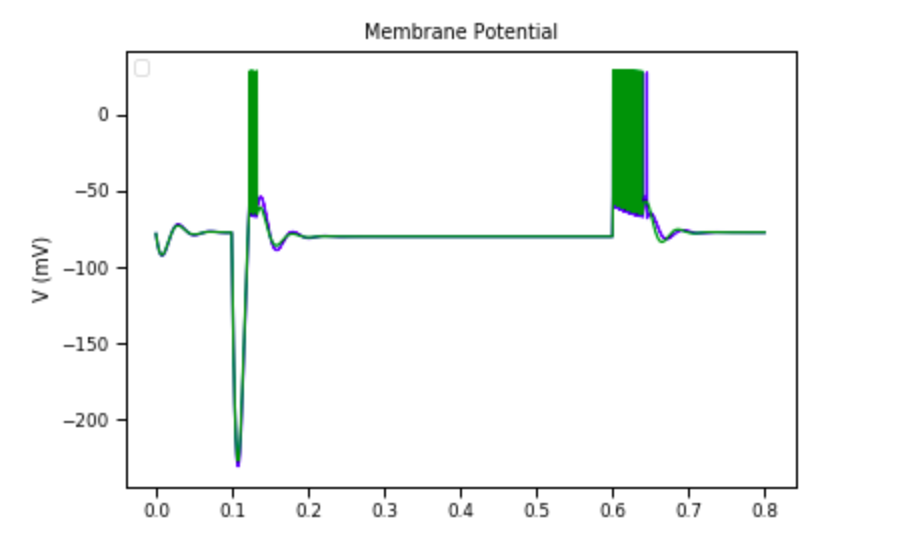
\includegraphics[scale=0.85]{figures/simulated_data_sub_threshold.png}
    \caption[Optimizer verification example 3]{\textbf{Optimizer Verification Example 2.}
    Similar to Figure
    \ref{fig:optimizer-verification-traces-2}, but for the AdEx model.
    Because model parameters are assigned to the ground truth model randomly, an unsually small value of $C$ in the AdEx model produces rebound spikes and bursts.
    This demonstrates that the match between the ground truth model and the optimized model is not limited to a single stimulus condition or exclusively to only typical model parameters.}
    \label{fig:adexp_model_rebound_spike}
\end{figure}

In these results, only a small number of features were used (Time Constant, Capacitance, Rheobase, Resting Potential, Input Resistance, and FISlope); interestingly only two of these involved a measurement of action potentials.
Other NeuronUnit tests that measure and judge models according to action potential \emph{Width, Amplitude, or Threshold} did not participate in guiding optimization, for reasons that will be described in Section \ref{sec:contingent_discontinous}.

%% No, this is not the reason.
% because many reduced models simply cannot produce realistic looking waveforms without imputation -- currently false, actually AP shape is fine in these versions of Izhikevich and Adex and they have been shown to achieve experimental agreement in those measurements.
% The reason is the corrogations/ripples I have been talking about for the last while.

%The AdExp model, for example, is far from an arbitrary waveform generators.
Results for additional models and parameterizations are given in the Appendix.

Failure of optimization verification, when it occurs, could be indicative of insufficient constraints.
By analogy, when solving a system of linear equations, finding a unique solution requires that the number of constraining equations is greater than the number of free variables you are solving for.
Similarly, in a genetic optimization algorithm we solve for unknown variables using stochastic principles, but the number of variables (i.e. model parameters) we can identify is still limited by the number of independent measurements of model output that we use.
In other words, assuming that the number of objectives in the multiobjective optimization problem, $NOBJ$ is greater than $NDIM$, the number of model parameters, optimization should be achievable.
Even when $NOBJ<NDIM$, such as in the examples above, optimization can still work due to correlations or redundancies in the model that lead the actual manifold on which models live to be of lower dimension than $NDIM$ itself.

\subsection{Verification Efficiency}
My optimizer can recover ground truth models from simulated data in several cases.
Does it do so efficiently?
How long does this optimization take, and does it get stuck exploring irrelevant regions of parameter space?

In Figure \ref{fig:optimizer-evolution}, I show how the optimized model converges towards the ground truth model over time.
In can require up to $200$ generations of parameter set evolution for tight convergence to be realized.
This takes approximately $10-20$ minutes on a my personal laptop.

% I have not done this (since numba on Adex, and IZHI existed) so I don't know the times for HPC. can be accelerated $XXXX$-fold on HPC architecture. 

%\begin{comment}
%\begin{figure}
%    \centering
%  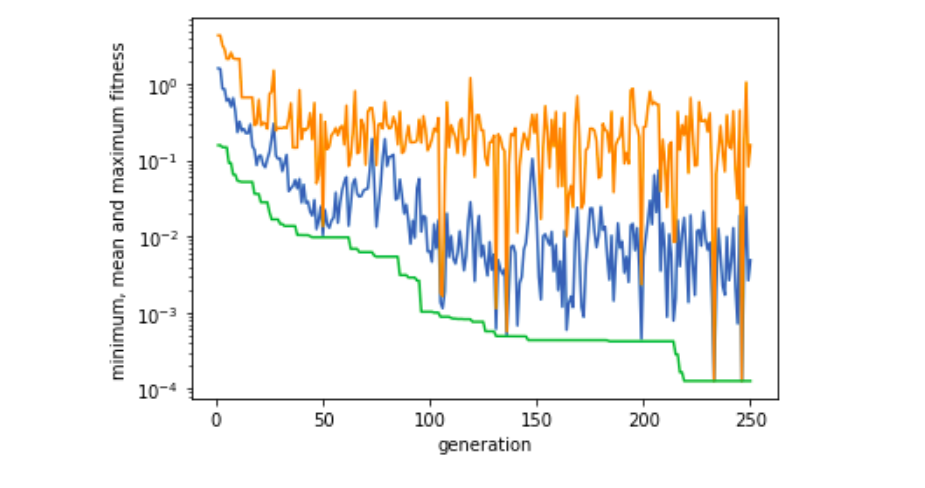
\includegraphics{figures/simulated_data_stats.png}
%    \caption{Optimizer evolution, green line tracks evolution of best fitness, blue line average fitness, %orange line is worst fitness. GA params, $NGEN=200$, $MU=50$,$cxp=0.3$,$mupb=0.2$ from this plot can see that %genes are storing and exploiting information, $cxp+mutpb=0.5$, so $50\%$ of genes are conserved between %generations }
%    \label{fig:my_label}
%\end{figure}
%\end{comment}

\begin{figure}
    \centering
    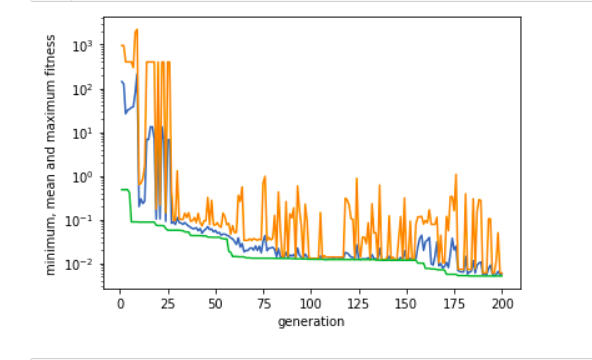
\includegraphics[scale=0.7]{figures/optimizer_internal_validation}
    \caption[Optimizer error over generations]{Evolution of optimized model quality over generations.
    The green line tracks the lowest error in each generation of candidate AdEx models, the blue line shows the average error, and orange line the highest error.
    Optimization hyperparameters were: Number of Generations=200, Population Size=50, Crossover Probability=0.3, Mutation Probability=0.2.
    The periodic jumps in the orange error represent mutation or crossover events in which poor-performing models were generated.
    These were not typically selected into the subsequent generation.
    Because the crossover and mutation probabilities only sum to 0.5, the remaining half of all parameter sets in each generation either filtered out by selection or, are simply carried over to the subsequent generation.
    Extensive hyperparameter tuning (not shown) demonstrated that this level of chromosome conservation was a good balance between exploration and exploitation.}
    \label{fig:optimizer-evolution}
\end{figure}

\subsection{Alternatives for Verification}
The ground truth is known independently of the optimizer, so one can test alternative strategies to see if there is a solution that represent a better match to ground truth than the one obtained through optimization.
For example, one can exhaustively search the solution space to look for the best model.
An exhaustive search might be a reasonable (but lazy) approach when there are only a small number of free parameters, however using a sampling grid of 25 distinct parameter values for each of N parameters mean that $25^{N}$ total models must be examined.
Even for a simple model ($N=5$) this represents nearly 10,000,000 model evaluations, and of course the problem gets much worse with each additional parameter.
25 values for each parameter may also be insufficient resolution when the parameter regime exhibiting the desired behavior is narrow.

\subsection{Implications of a verified optimizer}
Success here suggests that for reduced models, there is unlikely to be much degeneracy in model parameters, with distinct combinations of parameters producing identical simulated responses across a range of stimuli.
% Actually I did find some degenerecy, but I didn't find a way to systematically quantify it, because I spent too much time confounded by the ripple in surface problems.
This might also be expected from the motivation of reduced models, which is to identify and consolidate redundant or unimportant biophysical equations/parameters into a handful of key reduced model equations/parameters.
Importantly, I showed that the electrophysiological features used here, which correspond to measurements that can be made in real neurons, were sufficient for this task.

Confident that the optimizer can identify model parameterizations that can generate observed electrophysiological features \emph{in principle}, the focus of the remaining sections becomes the localization of other potential sources of model/data disagreement. 
